\documentclass[paper=a4,10pt]{scrartcl}

\usepackage[utf8x]{inputenc}
\usepackage[ngerman]{babel}
\usepackage[T1]{fontenc}

\usepackage{graphicx}
\usepackage{float}
\usepackage{subcaption}

\usepackage{fancyref}

\usepackage[numbers,square,sort]{natbib} %praktikumsquellenvorgabe
\usepackage{amsmath}
\usepackage{amssymb}

\usepackage{url}
\usepackage{hyperref}

\usepackage[a4paper, includehead, includefoot]{geometry}
\geometry{left=2cm, right=2cm, top=2cm, bottom=2cm}

%\usepackage{multibib}
\bibliographystyle{unsrt}


\title{Stochastik}
\author{Katrin Strassen, Robert Kummer}
\date{2019}

\begin{document}
\pagenumbering{gobble}
\maketitle
\newpage
\tableofcontents
\newpage
\pagenumbering{arabic}
\setcounter{page}{1}
\section{Grundbegriffe}
\subsection{Urbild}
Seien $A$ und $B$ zwei Mengen, $f: A \rightarrow B$ eine Funktion und $M$ eine Teilmenge von $B$. Die Menge
\begin{equation}
f^{-1}(M) := \{ x \in A \ | \ f(x) \in M \}
\end{equation}
wird Urbild von $M$ unter $f$ genannt. Das Urbild ist damit ein Wert der Urbildfunktion, die jedem Element $M$ der Potenzmenge $\mathcal{P}(B)$ das Urbild $f^{-1}(M)$ als Element der Potenzmenge $\mathcal{P}(A)$ zuordnet.\\

\noindent
\textit{In eigenen Worten: Die Funktion $f$ bildet Elemente von $A$ auf Elemente von $B$ ab. Das Urbild von einer Teilmenge $M \subset B$ ist die Teilmenge aller Werte aus $A$ die durch die Funktion auf Werte in $M$ abgebildet werden.}\\

\noindent
Für das Urbild von einelementigen Teilmengen schreibt man auch:
\begin{equation}
f^{-1}(\{b\}) := f^{-1}(b).
\end{equation}

\begin{figure}[h]
\centering
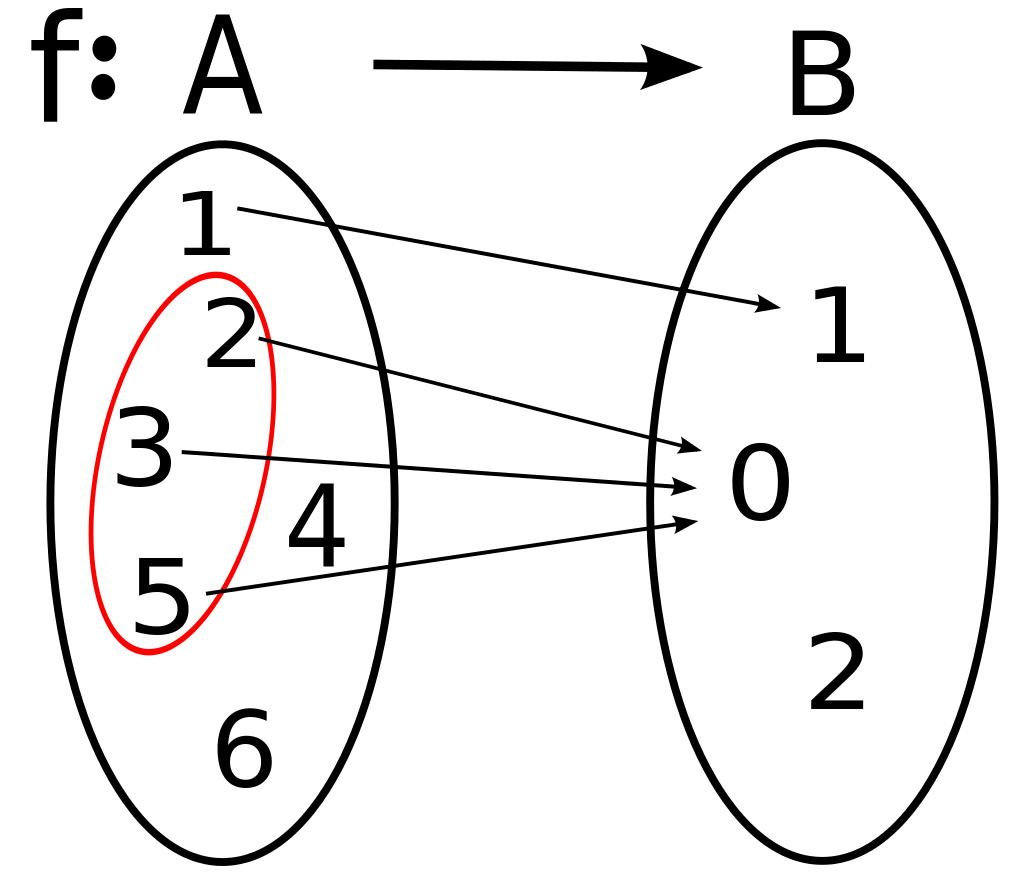
\includegraphics[width=0.4\textwidth]{../Bilder/urbild.png}
\label{urbild}
\caption{Beispiel: Das Urbild von $M=\{0\} \subset B$ ist $\{2,3,5\} \subset A$.}
\end{figure}

\subsection{charakteristische Funktion}
Gegeben sei eine bel. Grundmenge $X$ und eine Teilmenge davon $T \subset X$. Die Funktion $\chi_T: X \rightarrow \{0, 1\}$ definiert durch
\begin{equation}
\chi_T(x) = \begin{cases}
      1, & \text{falls}\ x \in T \\
      0, & \text{falls}\ x \not\in T \\
    \end{cases}
\end{equation}
heißt charakteristische Funktion oder Indikatorfunktion der Menge $T$.

\subsection{einfache Funktion}
Sei $(X, \Sigma)$ ein Messraum und $V$ ein (reeller, oder komplexer) Banachraum. Eine Funktion $u: X \rightarrow V$ heißt einfache Funktion, wenn folgende Bedingungen erfüllt sind:
\begin{itemize}
\item $u$ nimmt nur endlich viele Werte $\{ v_1, v_2, \dots, v_n\}$ an 
\item für alle $v \in V$ gilt $u^{-1}(\{v\}) \in \Sigma$, $u$ ist also messbar
\end{itemize}
Wenn auf $\Sigma$ noch ein Maß $\mu$ definiert ist, also ein Maßraum vorliegt, fordert man manchmal noch zusätzlich:
\begin{itemize}
\item $\mu(u^{-1}(V \setminus\{0\}))$ ist endlich
\end{itemize}

\noindent
Die Forderungen sind äquivalent zu der Aussage, dass $u$ die folgende Darstellung besitzt:
\begin{equation}
u(x) = \sum^n_{i=1}v_i \cdot \chi_{E_i}(x),
\end{equation}
wobei die $v_i \in V$ und $\chi_{E_i}$ die charakteristische Funktion der messbaren Menge $u^{-1}(\{v_i\}) \in \Sigma$. \\

\noindent
\textit{In eigenen Worten: Egal welches Argument $x$ man der Fkt $u$ übergibt, es muss ein Wert aus der endlichen Menge raus kommen. Messbarkeit wird in Sek. \ref{sec:messbar} behandelt, wobei hier nur gefordert wird, dass die Urbilder der Einelementmengen in $\Sigma$ liegen. Allgemein sollte das Kriterium für beliebige Teilmengen von $V$ gelten. In der letzten Forderung sieht es doch so aus, als wäre allgemeine Messbarkeit gefordert, da das Urbild einer mehr als ein Element großen Teilmenge von $V$ vom Maß angenommen werden und daher in $\Sigma$ liegen muss. Die letzte Forderung sagt aus, dass das Maß vom Urbild des Raumes ohne Null endlich sein soll. Also das Maß von der Teilmenge aller Elemente aus $X$, die durch $u$ auf $V \setminus \{ 0\}$ abgebildet werden, soll endlich sein. Mal sehen wofür man das fordert. Zu der äquivalenten Formulierung: Die charakteristische Funktion ist 1, wenn das x in der Teilmenge von $X$ liegt, welche durch $u$ auf $v_i$ abgebildet wird. Zur Summe trägt nur das $v_i$ bei, dessen Urbild unter $u$ das Argument $x$ enthält. Die Funktion nimmt damit nur Werte asu $V$ an, da die charakteristische Funktion nur einmal anschlägt und zwar genau dann, wenn das x im Urbild von einem bestimmten $v_i$ liegt. Da die Funktion eindeutig zuweist, liegt aber jedes x nur in einem Urbild und daher ist die charakteristische Funktion nur dann 1, wenn Urbild von einem best. $v_i$ und x zusammenpassen.}



\section{$\sigma$-Algebra}
Sei $\Omega$ eine nichtleere Menge und $\mathcal{P}(\Omega)$ die Potenzmenge dieser Menge. Eine Menge von Teilmengen $\mathcal{A} \subset \mathcal{P}(\Omega)$ (auch Mengensystem genannt) heißt $\sigma$-Algebra auf, oder über $\Omega$, wenn sie die folgenden drei Bedingungen erfüllt:

\begin{enumerate}
	\item $\mathcal{A}$ enthält die Grundmenge, also: $\Omega \in \mathcal{A}$
	\item $\mathcal{A}$ ist stabil bezüglich der Komplementbildung. Ist also $A \in \mathcal{A}$, dann ist auch $A^{\mathrm{C}} \in \mathcal{A}$.
	\item $\mathcal{A}$ ist stabil bezüglich abzählbarer Vereinigungen. Sind also die Mengen $A_1, A_2, A_3, \dots$ in $\mathcal{A}$ enthalten, so ist auch $\bigcup^\infty_{i=1}$ in $\mathcal{A}$ enthalten.
\end{enumerate}

\section{Wahrscheinlichkeitsmaß}
Gegeben sei eine Menge $\Omega$, die Ergebnismenge und eine $\sigma$-Algebra $\Sigma$ auf dieser Menge (das Ereignissystem).\\

\noindent
Dann heißt eine Abbildung
\begin{equation}
P: \Sigma \rightarrow [0,1]
\end{equation}
Wahrscheinlichkeitsmaß, wenn sie die folgenden Bedingungen erfüllt.

\paragraph{Normiertheit:}
\begin{equation}
P(\Omega) = 1
\end{equation}

\paragraph{$\sigma$-Additivität:}
Für jede abzählbare Folge von paarweise disjunkten Mengen $A_1, A_2, A_3, \dots$ aus $\Sigma$ gilt
\begin{equation}
P\left( \bigcup^{\infty}_{i=1}A_i\right) = \sum_{i=1}^{\infty} P(A_i). 
\end{equation} 

\noindent
Es gilt also, dass die Wahrscheinlichkeit für die Vereinigung zweier Ereignisse gleich groß ist wie die Summe der Einzelwahrscheinlichkeiten der Ereignisse.

\section{Wahrscheinlichkeitsraum}
Sei $\Omega$ eine beliebige \textbf{Ergebnis}menge. Sie umfasst alle möglichen Ergebnisse von einem Zufallsvorgang. Beim Würfeln ergibt sich also beispielsweise $\Omega = \{ 1,2,3,4,5,6\}$.

\noindent
Nun wird $\Sigma$ als eine $\sigma$"=Algebra über $\Omega$ definiert. Die Elemente von $\Sigma$ werden auch Ereignisse genannt. 

\noindent
Als letztes wird ein Wahrscheinlichkeitsmaß $P: \Sigma \rightarrow [0,1]$ benötigt. Das Tripel $(\Omega, \Sigma, P)$ ist dann ein Wahrscheinlichkeitsraum.
 

\section{Messraum}
Ein Tupel $(\Omega, \Sigma)$ heißt Messraum, wenn $\Omega$ eine beliebige Grundmenge ist und $\Sigma$ eine $\sigma$-Algebra über $\Omega$ ist.

\noindent
In der Stochastik wird der Messraum auch Ereignisraum genannt und ist einfach ein Wahrscheinlichkeitsraum ohne Wahrscheinlichkeitsmaß.

\noindent
Eine Menge $S$ wird messbare Menge genannt, wenn $S \in \Sigma$ gilt.

\section{messbare Funktion} \label{sec:messbar}
Seien $(\Omega_1, \Sigma_1)$ und $(\Omega_2, \Sigma_2)$ zwei Messräume. Eine Funktion $f: \Omega_1 \rightarrow \Omega_2$ wird $\Sigma_1$"=$\Sigma_2$"=messbar genannt, wenn für alle $S_2 \in \Sigma_2$ gilt, dass das Urbild von $S_2$ unter $f$ ein Element aus $\Sigma_1$ ist:
\begin{equation}
f^{-1}(S_2) \in \Sigma_1.
\end{equation}

\noindent
\textit{In eigenen Worten: Aus Wahrscheinlichkeitssicht: Die Funktion $f$ bildet Ergebnisse aus $\Omega_1$ auf Ergebnisse in $\Omega_2$ ab. Wenn ich mir ein Ereignis $S_2$ aus $\Sigma_2$ nehme, also eine Teilmenge von $\Omega_2$, müssen alle Ergebnisse aus $\Omega_1$, die durch die Funktion $f$ auf Ergebnisse von $S_2$ abgebildet werden, zusammen ein Element von $\Sigma_1$ sein. \\
Das muss für alle $S \in  \Sigma_2$ gelten. Egal, welches Ereignis $S$ aus $\Sigma_2$ betrachtet wird, das Urbild von $S$ unter $f$ muss ein Element von $\Sigma_1$ sein. Zu jedem Element $S$ der $\sigma$"=Algebra $\Sigma_2$ muss es ein Element von $\Sigma_1$ geben, das das Urbild von $S$ unter $f$ ist.}

\section{Zufallsvariable}
\subsection{Definition}
Eine Zufallsvariable (ZV) ist eine messbare Funktion von einem Wahrscheinlichkeitsraum in einen Messraum. Seien also $(\Omega, \Sigma , P)$ ein Wahrscheinlichkeitsraum und $(\Omega', \Sigma')$ ein Messraum. Eine $\Sigma$"=$\Sigma'$"=messbare Funktion $X:\Omega \rightarrow \Omega'$ heißt dann eine $\Omega'$"=Zufallsvariable auf $\Omega$.

\paragraph{Beispiel:} Es soll das Experiment des zweimaligen Würfelns mit einem fairen Würfel betrachtet werden. Der dazugehörige Wahrscheinlichkeitsraum $(\Omega, \Sigma, P)$ sieht wie folgt aus:

\begin{itemize}
\item $\Omega = \{ (1,1), (1,2), \dots, (6,5), (6,6) \}$ ist die Ergebnismenge aller möglichen Ergebnisse
\item $\Sigma = \mathcal{P}(\Omega)$ ist die Potenzmenge von $\Omega$
\item $P$ ist das Wahrscheinlichkeitsmaß. Da die Würfe unabhängig sein sollen, sollen alle 36 möglichen Ergebnisse gleich wahrscheinlich sein. Daher gilt: $P(\{ n_1, n_2\}) = \frac{1}{36}$ für $n_1, n_2 \in \{ 1,2,3,4,5,6\}$
\end{itemize}

\noindent
Es sollen nun zwei Zufallsvariablen definiert werden. Die ZV $X_1$ für das Würfelergebnis des ersten Würfels und eine andere $X_2$ für die Summe der beiden Augenzahlen.

\begin{itemize}
\item $X_1: \Omega \rightarrow \mathbb{R}; \qquad (n_1, n_2) \mapsto n_1$
\item $X_2: \Omega \rightarrow \mathbb{R}; \qquad (n_1, n_2) \mapsto n_1 + n_2$
\end{itemize}
Dabei wurde für $\Sigma'$ die borelsche $\sigma$"=Algebra auf den reellen Zahlen gewählt.

\subsection{Verteilung einer Zufallsvariablen}
Sei $X$ wieder eine ZV von $(\Omega, \Sigma, P)$ in den Ereignisraum $(\Omega', \Sigma')$. Dann heißt die durch
\begin{equation}
P_X(A') := P(X^{-1}(A')) \qquad \text{für alle }A' \in \Sigma' 
\end{equation}
definierte Abbildung $P_X: \Sigma' \rightarrow [0, 1]$ die Verteilung der Zufallsvariablen $X$ unter $P$. Hierbei bezeichnet $X^{-1}(A')$ das Urbild von $A'$ unter $X$, also das Ereignis
$\{ \omega \in \Omega \ | \ X(\omega) \in A' \} \in \Sigma$. \\

\noindent
\textit{In eigenen Worten: Die Wahrscheinlichkeit für ein Ereignis $S'$ aus $\Sigma'$ ist also die Wahrscheinlichkeit für das Ereignis $S = X^{-1}(S')$, das durch die ZV $X$ auf $S'$ abgebildet wird. Dazu braucht man auch die messbare Funktion $X$, da so die Urbilder für alle Ereignisse in $\Sigma'$ immer in $\Sigma$ liegen.}

%\section{Übergangskern}
%Man hat zwei Messräume $(\Omega_0, \Sigma_0)$ und $(\Omega_1, \Sigma_1)$. Eine Abbildung $K: \Omega_0 \times \Sigma_1 \rightarrow [0, \infty)$ heißt Übergangskern von $(\Omega_0, \Sigma_0)$ nach $(\Omega_1, \Sigma_1)$, wenn gilt:

%$\bullet$ Für jedes $x \in \Omega_0$ ist $K(x,\ \cdot \ )$ ein Maß auf $(\Omega_1, \Sigma_1)$.

%$\bullet$ Für jedes $S \in \Sigma_1$ ist $K(\ \cdot \ , S)$ eine $\Sigma_0$-messbare Abbildung.



\end{document}